\documentclass[]{scrreprt}
\usepackage{glossaries}
\usepackage{listings}
\usepackage[]{graphicx}

\newglossaryentry{latex}{
  name=LaTeX,
  description={Ein Textsatzsystem}
}
\newglossaryentry{consumer}{
    name=Consumer,
    description={A program using a UaDI conform DLL to get generated data from a producer or device}
}
\makeglossaries


\begin{document}

\chapter{The Idea of OmniView}
OmniView is planned to be an omniscient data-visualization and analysis tool. 
OmniView itself shouldn't need to know anything about any given data-producer at compile-time, but should still be able to visualize the produced information.
OmniView itself shouldn't need to know anything about any given analysis-tool at compile-time, but should still be able to use an analysis-API. 
In order for OmniView to work this way, there shall be a structured architectural approach, to enable modular development.
This includes dataproducer devices as well as analysis-tools.

\section[Modules]{Modules of OmniView and their Role}
The Name OmniView actually only applies to the executable instance, that is in charge of displaying gathered data in a way similar to PicoScope or sigrok, whether it's live or archived data. 
Since (well-designed) modularity can help keeping the complexity of a system in check, the greater OmniView-Architecture is a project of the Bochumer AI-Group.
\\
A oscilloscope-like user-interface is the most generic way, to display data as a function over time. 
All measurement-values are a sample of a certain unit (sometimes even an SI-Unit) at a specific point in time, and thus projectable onto a plane with its unit in y- and the time in x-dimension. 
Displaying a multitude of different y-dimensions in an oscillogram is a well-proven design and has been implemented in several data-recorder software-suites. 
\\
Incoming live-data into the view is delivered via a websocket connection.
There won't be hard real-time guarantees in this interface. 
This websocket is provided by an entity that implements the concept of an epoch-server.
Soft real-time can be guaranteed to a certain extend in the internal structure of the epoch-server and its storage-interface.
Due to the nature of live-updates of a GUI, new updates are being received on a regular basis and prepended to the n-1 dataset.
Each update-object that contains data to be prepended, and displayed in the oscillogram is called a column. 
It derives its name from the property, that it holds several values of different data-channels in parallel.
The aggregation to a continuous stream of such pieces of information that belong to one channel is called a waveform. 
\\
An epoch-server has the ability to maintain multiple websocket connections, and an OmniView-Instance has the ability to maintain connections to multiple epoch-servers. 
Before a view can instantiate a connection with a websocket, it queries the epoch-servers REST-API, to receive a structure know as possibility-list.
This list contains all available devices, and all available transducers. 
A transducer is a function that works as a filter.
It implements a directed node, taking one or more waveforms as an input and having exactly one waveform as an output. 
Using transducers, a so-called (processing-)route can be constructed. 
A route is a directed graph composed from transducer-nodes. 
For further investigation see \ref{chap:WaveformProcessingNetwork}.
The structure inside the epoch server that defines which channels are being send out to a specific connection is called the connections visibility-list. 
This list in combination with a checkbox will also be displayed in the view.

\begin{figure}
    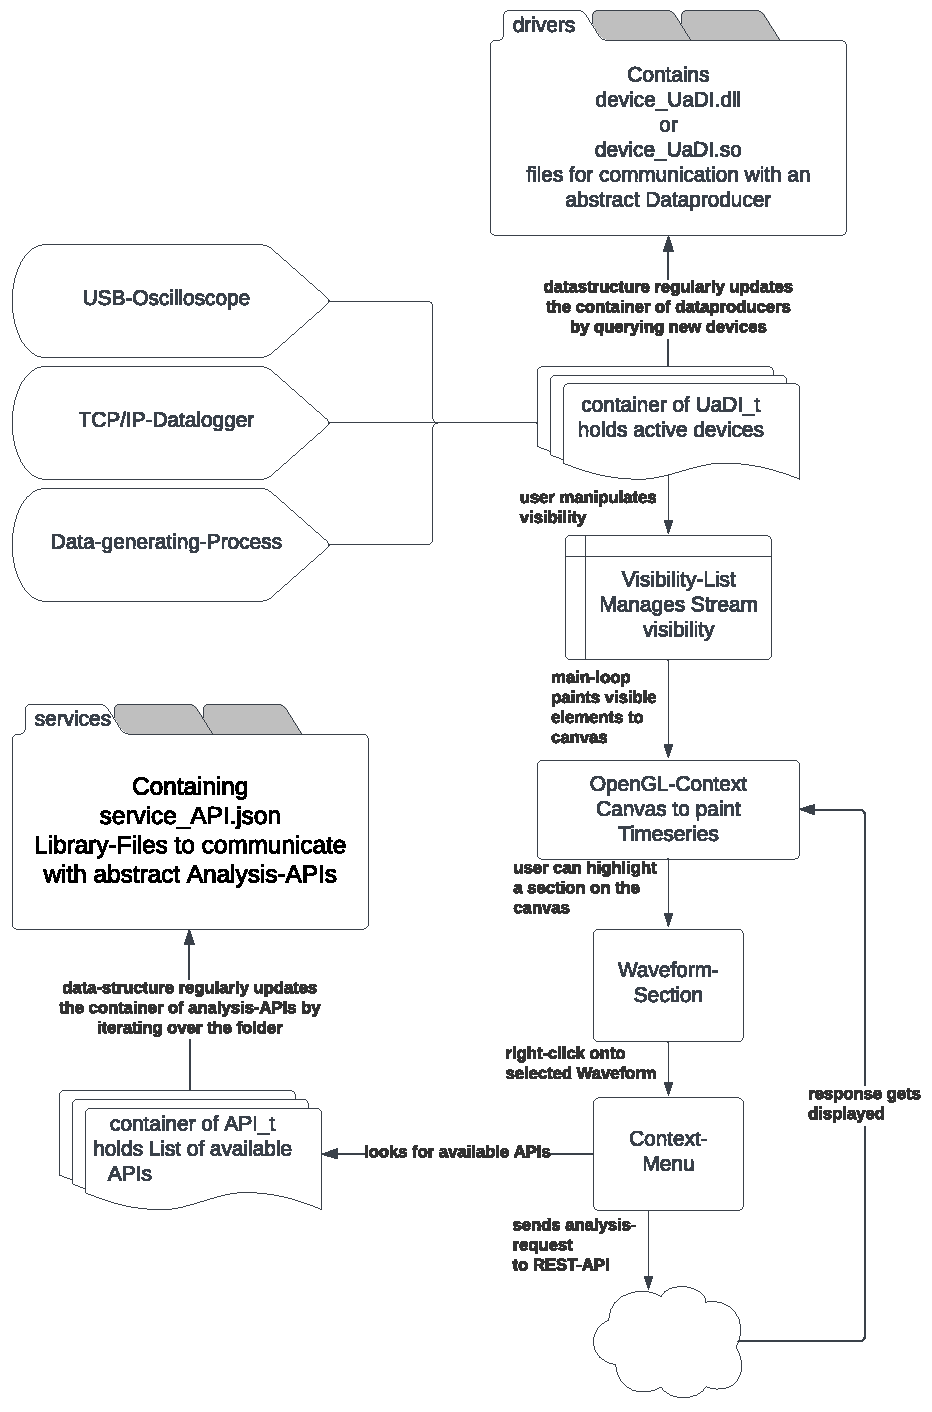
\includegraphics[width=.9\textwidth]{./assets/pictures/overview.pdf}
    \caption{Overview of Modules}
    \label{fig:Overview}
\end{figure}

\section[Greater Picture]{OmniView and its Role in the Greater Picture}
Auto-Intern GmbH and their connected entities have been working on a unified architecture for measurement- and monitoring-devices since the early 2000s. 
Integrating measurement-systems into larger architectures is by no means a trivial task.
OmniView fits into the Grand-Unified-Monitoring-Architecture of Auto-Intern.


\begin{figure}
    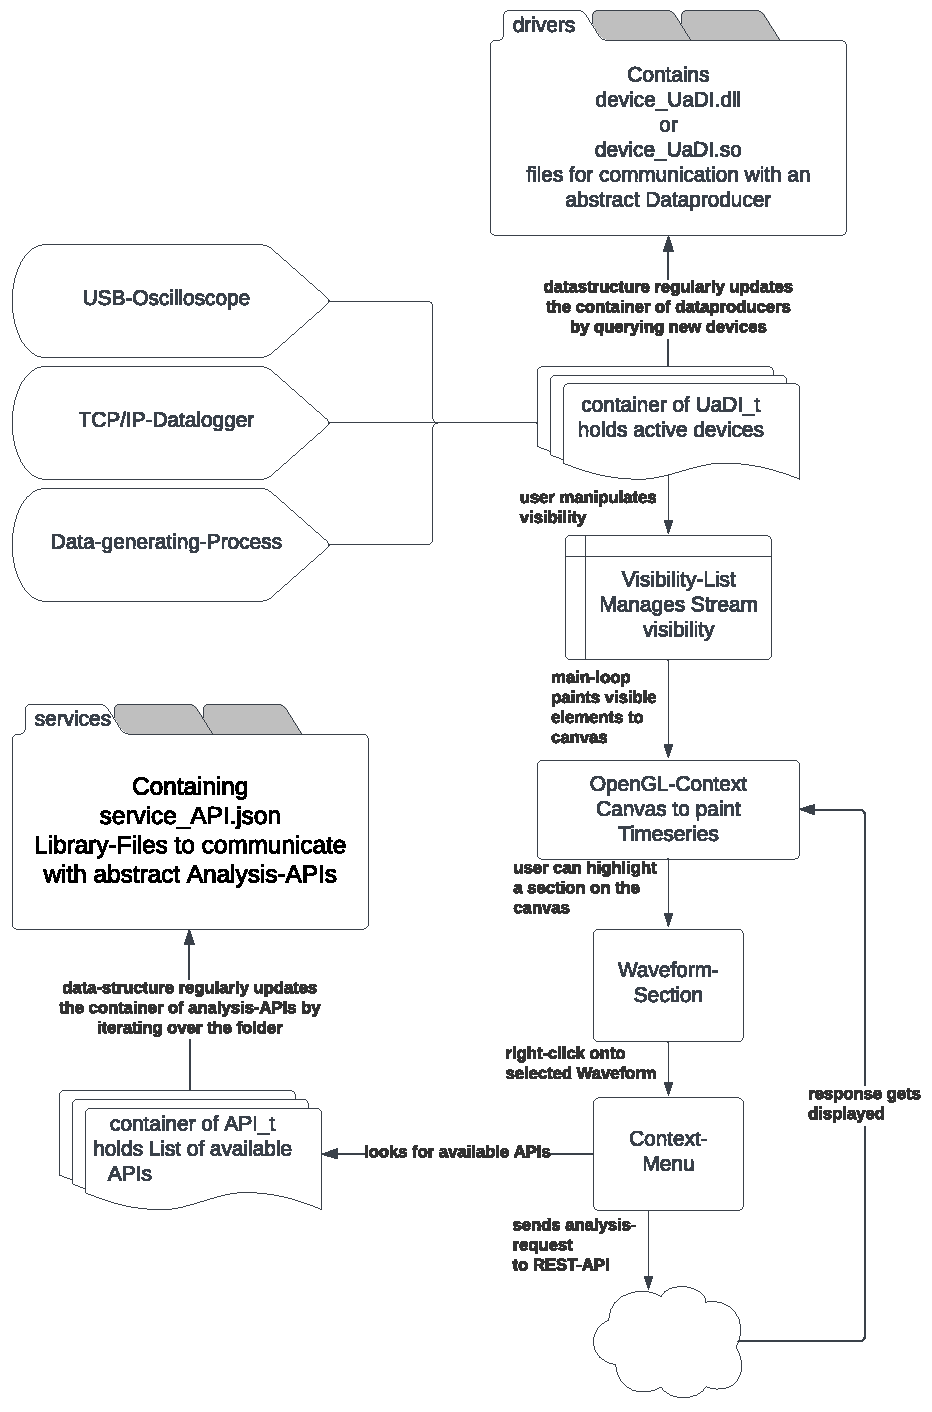
\includegraphics[width=.9\textwidth]{./assets/pictures/overview.pdf}
    \caption[]{Brief overview of the proposed structure}
    \label{fig:overview}
\end{figure}


There shall be a unified way to interact with an abstract data-producer.
This includes devices such as:
\begin{enumerate}
    \item a USB-oscilloscope \gls{latex}
    \item a TCP/IP client, sending a continuous stream
    \item a USB-logic-analyzer
    \item a random-number-generator
    \item a filedescriptor
\end{enumerate}

Since it is not known at compile-time, which devices will be used at runtime, the code can't be linked statically into OmniView (or any other data-\gls{consumer} for that matter). 
Therefor an interface shall be defined, that gets used by the consumer, but the implementation of the data-handling ought to be provided in a dynamically linked library. 
From here on forward we will refer to this as \lstinline|DLL| even though \lstinline|.dll| and \lstinline|.so| are meant equally. 
If a windows \lstinline|.dll| or a linux \lstinline|.so| is meant specifically, please use the terms \lstinline|.dll| or \lstinline|.so|, otherwise \lstinline|DLL|. 
Be aware, that this \lstinline|DLL| does not necessarily constitue an aquivalent to an actual device-driver with a communication-channel to the systems kernel.
\\
It appears, that all dataproducers that are relevant for OmniView can be abstracted in a certain way, and thus share the same function-calls in a \lstinline|DLL|.
There are three requirements:
\begin{itemize}
    \item Grabbing the next part of the data-stream asynchronusly
    \item The data-producer providing meta-information about itself 
    \item Send control-data from the consumer to the data-producer
\end{itemize}
This interprocess-communication comes with some additional hurdles.

\section{Memory Management Ideology}
Not only does OmniView not know about which devices will be connected at runtime, it also does neither know about the amount of devices that will be attached, nor does it know what data-rate the producers will provide.
Due to this uncertainties, a strongly structured memory allocation ideology needs to be implemented in order to minimize error-prone sections in the applications code.


\section[UaDI]{Unified abstract Data\-producer Interface}
The \textit{Unified abstract Data\-producer Interface} is the protocol that specifies the interprocess\-communication between the con\-sumer and the device, using the \lstinline|DLL|. 

\begin{figure}
    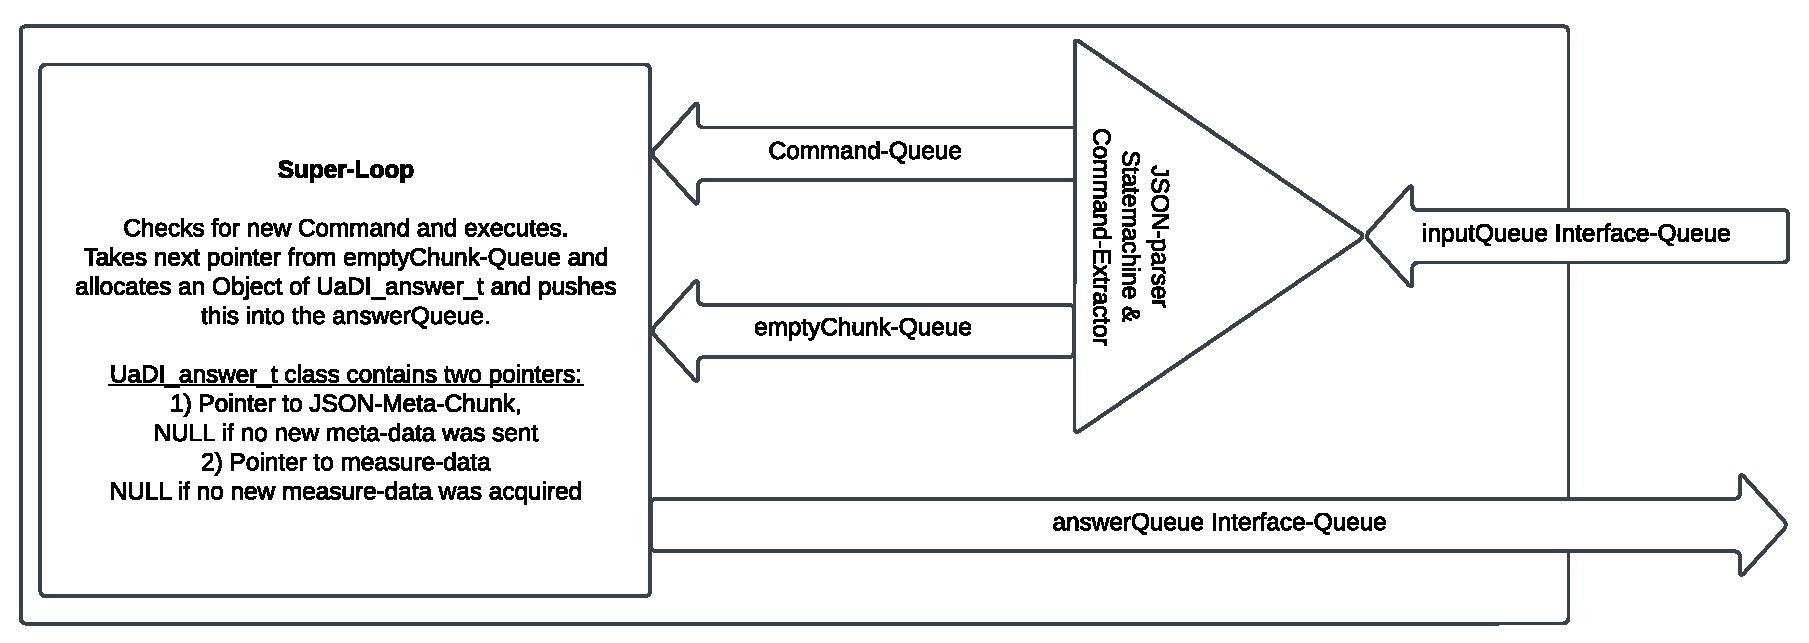
\includegraphics[width=.9\textwidth]{./assets/pictures/interface.pdf}
    \caption[]{Coarse structure of the DLL-interface}
    \label{fig:dllinterface}
\end{figure}


\chapter{Dataproducers}
The origin of a stream of measurement-samples is called a device, as refered to in the UaDI specification. 
A device may get control-input, but always has to back-channels to a consumer:
\begin{itemize}
    \item a pointer to a JSON chunk
    \item a pointer to a data chunk
\end{itemize}
\section{Memory-Management}
A device doesn't allocate on its own.
Therefor it needs to get a memory-pointer from the consumer.
The so called chunks are of a default size of 128*1024 bytes.
Pointer to these memory-locations are known as chunk\_ptr.
The consumer is responsible for the memory management of these chunks.
An array of chunk\_ptr can be handed to the device on claiming it, as well as through a routine called uadi\_push\_chunk.
In both cases, the consumer passes an array of chunk\_ptr, and the amount of chunk\_ptr to the device.
When claiming the device, a callback is also registerd. 
The callback is called, when the device is finished with writing into a chunk.
The callback is called with a chunk\_ptr and a void pointer to the consumers context. 
The device doesn't care about the context pointer, it just hands it back to the consumer.
Which data-type the device hands back is defined by the device. 
In the first usecases, only float shall be supported. 
The data-type will be handled in a second layer on top of UaDI, that performs device-management.

\section{Concrete Devices}
There are several devices already planned that need to be supported by the end of 2024:
\begin{enumerate}
    \item OmniScope - USB-Single-Channel Oscilloscope
    \item OmniScope Duo - USB-Dual-Channel Oscilloscope
    \item OmniEField - USB-E-Field Probe
    \item OmniBField - USB-B-Field Probe
    \item OmniTherm - USB-Thermocoupler Typ-K 
    \item OmniPower - USB-Power-Monitor
    \item OmniPower ETH - Ethernet-Power-Monitor
    \item OmniSonic - USB-Vibration-Sensor
    \item AI PowerProbe - Ethernet E-Field/B-Field Probe 
    \item Random Number Generator Software-Device
    \item IOTA Software Device 
    \item PCIe - Generic Integer Kintex7 FPGA Device
\end{enumerate}

\chapter{The Waveform-Processing-Network}
\label{chap:WaveformProcessingNetwork}
A transducer is a directed node, and serves the function of forwarding and manipulating a value of a given waveform.
Routes are directed graphs, consisting of nodes of transducers and attributeless connections between them.
Routes can be dynamically constructed. 
The Waveform-Procesing-Network it is a global singleton static object, that gets default-constructed at the epoch-servers startup, and offers the routines .addRoute(Route\_t\&\& newRoute).
These transducer-nodes might take additional construction parameters. 
A route is to be read from right to left, since the interpretation can be ambigious reading from left to right. 
Routes can be configured via a REST-API POST method, that adds a specific route to a connection. 
\chapter[Further Devl]{Further Development of OmniView}
OmniView as it is right now has a limited shelf-life. 
The current version will be deprecated somewhere around summer of 2024.
It will be replaced by a more modular approach, that consists of two separate pieces, called OmniDaemon and OmniView 2.0.
OmniView 2.0 will be written in Angular.
OmniDaemon will still be written in C++ and use the same approach for data-acquisition. 
The interprocess-communication between the data and the view on the data will be implemented by using websockets for live-streaming, REST for settings and downloading whole files and MQTT-Publishing for sending out alarms and similar fire-and-forget messages. 

\section{User Interface}

The following chapters describe the user interface of the omnAIView application, providing a detailed overview of its various components and their functionality. The design of these components is also introduced here, while a more thorough explanation of the design principles can be found in Chapter \ref{cap:Designprinciples}. All components should adhere to these principles. If there are any questions after reading the description, they can be added as issues for the FAQ.

The user interface is currently implemented in C++, with plans to transition to JavaScript in a subsequent phase. This interface serves as a central hub for configuring connected devices, conducting measurements, saving data in various formats, displaying and analyzing the acquired data. Additionally, users can access an integrated Help Menu that directs them to a website providing comprehensive information about omnAIView and omnAIScope.

The application is divided into four main regions: the Toolbar, the Sidebar Menu, the Plot Region, and the Devices Menu.

\subsection{Basic Interface}

The basic interface includes:
\begin{itemize}
\item A top bar featuring the company name, a save button, and start/stop measurement buttons.
\item An adjustable window where data is displayed.
\item A sidebar for:
    \begin{itemize}
    \item Searching devices
    \item Loading old data
    \item Diagnostics
    \item Settings
    \item Help
    \end{itemize}
\item A bottom window, which can be minimized, displaying connected devices and loaded data files.
\item Several popup windows for functions such as analysis.
\end{itemize}

The size of the GUI should adapt to the screen size being used. The design is illustrated in Figure \ref{fig:GUI}.

\begin{figure}[!h]
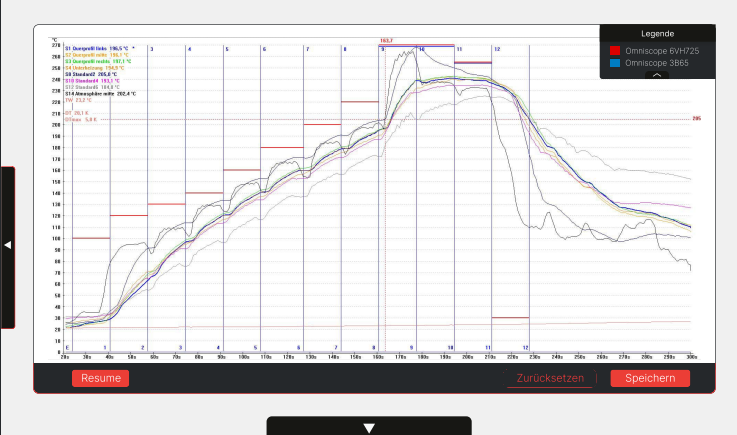
\includegraphics[width=.9\textwidth]{./assets/pictures/DatawindowVersion1.0.png}
\caption[]{A visual representation of the GUI interface with all menus selected}
\label{fig:GUI}
\end{figure}

The language displayed in the pictures is German.

Popup windows include:
\begin{itemize}
\item A window to load old data from the filesystem into the application.
\item A window to save the measured data.
\item A window to generate training data from loaded or measured data.
\item A window to analyze loaded or measured data.
\item A settings window.
\end{itemize}
This list is not exhaustive.
 All popup windows should follow the same structure and design principles, which can be found in Chapter \ref{cap:Designprinciples}. 
 An example of a popup window is shown in Chapter \ref{cap:Designprinciples_Popupwindows}.

\section{Toolbar}

The toolbar, displayed at the top of the program, contains the company logo on the left side, 
a save button on the right side, and start/stop measurement buttons as well as a reset button in the middle. 
The specific placement of the start and stop buttons is still under consideration. A visual representation of the toolbar is shown in Figure \ref{fig:toolbar}.

\begin{figure}
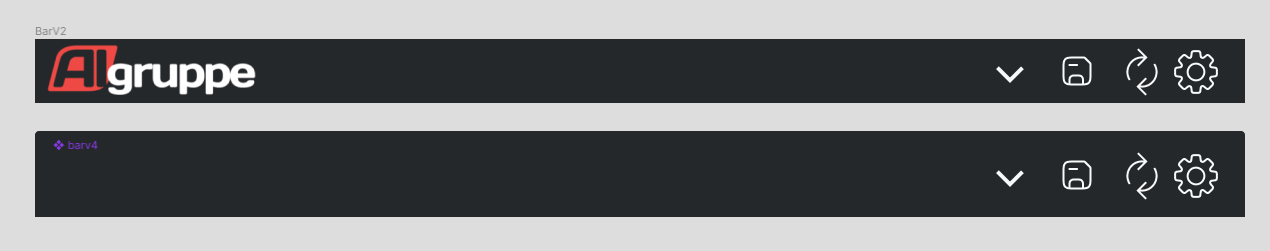
\includegraphics[width=.9\textwidth]{assets/pictures/Toolbar states.png}
\caption[]{A visual representation of the toolbar with different buttons}
\label{fig:toolbar}
\end{figure}

\subsection{Save Button}
The save button, designed as an icon button according to the principles in Chapter \ref{cap:Designprinciples_PopupButtons},
 writes the measurement (a waveform stack) to storage. The storage options include the computer's file system, a Database Management System (DBMS), or a Cloud platform.

\subsubsection{User Story for the Save Button}
\begin{itemize}
\item \textbf{Visibility Before Measurement:} The save button should be prominently visible.
\item \textbf{Greyed-out During Measurement:} While the measurement is in progress, the save button should appear greyed out.
\item \textbf{Post-Measurement Access:} Upon completion of the measurement, the save button should be accessible.
\item \textbf{Prompt Save Window:} Clicking the save button should open a window designed according to the principles in Chapter \ref{cap:Designprinciples_PopupWindow}.
 A visual representation of the save window is shown in Figure \ref{fig:SavingWindow}.
\end{itemize}

\begin{figure}
    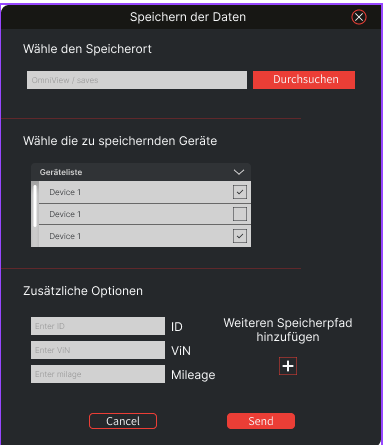
\includegraphics[width=.9\textwidth]{assets/pictures/Popupwindow_png.png}
    \caption[]{A visual representation of the Popupwindow: Saving}
    \label{fig:SavingWindow}
    \end{figure}

\subsubsection{Save Window}
The save window is divided into four sections:
\begin{itemize}
\item \textbf{Saving Path:} Users can choose a default path, manually enter a path, or select a path using a file browser.
\item \textbf{Device Selection:} Users can select devices to save via a drop-down menu.
\item \textbf{Additional Information:} Users can input the vehicle information (VIN, mileage) and select a vehicle type. Additionally they can input a measurement name.
\item \textbf{Save or Cancel:} Users can either save the settings or cancel the menu. The data should be saved under the input path, as measurementname_omnAIscopeID. 
\item \textbf{Saved file:} The saved file should be a .csv file. In the first line the metadata as well as the omnAIScopeID and the sampling rate should be saved. 
                            Under that the waveform should be saved. 
\end{itemize}

\subsection{Reset Button}
The reset button resets all measurements and reloads all connected devices. When pressed, a rotating symbol should appear until the app reconnects the devices and resets the data.
This should not reset the data that was loaded extern. 

\subsection{Start/Stop Button States}
The specific placement of the start and stop buttons, whether in the toolbar or plot region, is still under consideration.

\section{Plot Region}

The plot region displays the data window where measurements are shown.
 It is positioned in the middle of the screen and adapts to the opening and closing of the devices list or sidebar menu. 
 A visual representation of the data window is shown in Figure \ref{fig:datawindow}.

 The axis of the data window adapt to the connected device. The axis show the devices measurement unit on the y-axis as well as the time in seconds on the x-axis. 
 If more than one device with different measurement units is connected, there will be additional y-axis that can be edited seperately.

\begin{figure}
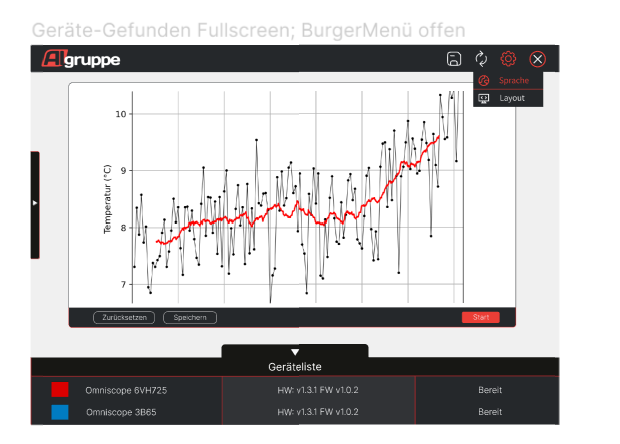
\includegraphics[width=.9\textwidth]{assets/pictures/Mainwindowopen.png}
\caption[]{A visual representation of the data window with a legend}
\label{fig:datawindow}
\end{figure}

While a measurement is being taken, the scale and size of the data window cannot be changed. After the measurement, the user can adjust the data window, including:
\begin{itemize}
\item Zooming in and out on both axes.
\item Adjusting the scale of the x- and y-axes.
\item Selecting and displaying a specific part of the data window.
\end{itemize}

Adjustments can be made using a mouse, mousepad, touchpad, or keyboard shortcuts. The user can also export the data window as a PDF.

\section{Sidebar Menu}

The sidebar menu, located on the left side of the application, can be expanded and closed via a side button. It contains five submenus, each with its own icon:
\begin{itemize}
\item Searching devices ("Suche Geräte")
\item Loading old data ("Daten hinzufügen")
\item Diagnostics ("Diagnose")
\item Settings ("Einstellungen")
\item Help ("Hilfe")
\end{itemize}
A visual representation of the sidebar menu is shown in Figure \ref{fig:sidebarMenu}.

\begin{figure}
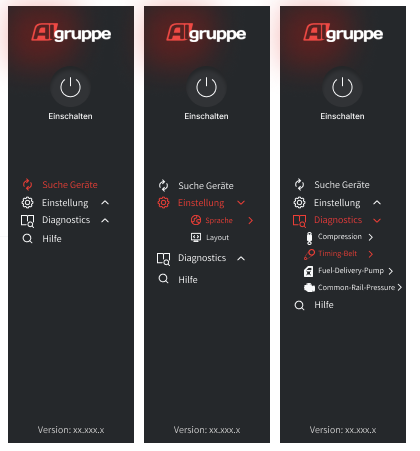
\includegraphics[width=.9\textwidth]{assets/pictures/SideBarMenu.png}
\caption[]{A visual representation of the sidebar menu in its different states}
\label{fig:sidebarMenu}
\end{figure}

\subsection{Searching Devices}
The "Searching Devices" submenu contains a button that, when clicked, searches for connected devices. Found devices are displayed in the devices list menu, and connected OmnAIScopes light up in
different colors.

\subsection{Loading Old Data}
The "Loading Old Data" submenu contains a button that opens the "Load Old Data" popup window. Configurations for this popup window are detailed in Section \ref{cap:PopupWindow_loadoldata}.

\subsection{Diagnostics}
The Diagnostics button opens a popupwindow with options for different analyses or generating training data. The popupwindow and its functionality is described in section \ref{cap:Diagnostics}.

\subsection{Settings}
The Settingsbutton opens a popupwindow "Settings menu" described in Section \ref{cap:PopupWindow_settings}.

\subsection{Help Menu}
The Help button directs users to a website. Before accessing the website, a popup window asks for confirmation.

\section{Popup Windows}

This section describes the configuration and functionality of the various popup windows.

\subsubsection{Popup Window: Settings} \label{cap:PopupWindow_settings}

The Settings popup window allows users to customize the appearance and configuration of the OmnAIView interface. This window is divided into several sections:

\textbf{Setting ID}
\begin{itemize}
    Users can set their ID by writing it into the Input field. There should be a disclaimer that the ID can only be set once. 
    The ID will be written into the config. 
\end{itemize}

\textbf{Language options}
\begin{itemize}
    Users can choose between different languages. Currently available are English and German. 
\end{itemize}

\textbf{Graphical options}

The following point should be in a TreeNode \textbf{Graphical Settings} [grafische Einstellungen]
\textbf{Theme Selection:}
\begin{itemize}
    \item Users can choose between different themes such as Light and Dark. Each theme should be visually distinct to accommodate various user preferences and needs.
\end{itemize}

\textbf{Font Settings:}
\begin{itemize}
    \item This section includes options to change the font type, size, and color. Users can preview the font changes in a sample text box before applying them.
\end{itemize}

At the end of the menu there is a save, back and rest button. The reset button allows users to revert all settings to the default configuration if needed. The back button will not change any settings.
The saves button applies the settings and saves them in the config, so the settings are still this way when the user opens the application again. 

\textbf{Reset to Default:}
\begin{itemize}
    \item 
\end{itemize}

\subsubsection{Popup Window: Load Old Data} \label{cap:PopupWindow_loadoldata}

The Load Old Data popup window first contains only one inputfield , a browse button right to it as well as a \textbf{Load all data} and back button. 
It provides three options for importing previously collected data:

\textbf{1. Manual Path Input:}
\begin{itemize}
    \item Users can manually enter the file path where the old data is stored in the input field.
    A text input field labeled "Path" is provided for this purpose.
     Above the input field, there is a text "Enter the path to your data" (Geben Sie den Pfad zu Ihren Daten ein).
\end{itemize}

\textbf{2. Browse Button:}
\begin{itemize}
    \item Users can also click on a "Browse" (Durchsuchen) button to open a file explorer window and navigate to the desired file location.
     The selected path is then displayed in the text input field.
\end{itemize}

\textbf{3. Drag and Drop:}
\begin{itemize}
    \item Alternatively, users can drag and drop a file directly into the application.
     A designated area labeled "Drag and drop your file here" (Ziehen Sie Ihre Datei hierher) is clearly marked in the window.
\end{itemize}

If the user wants to enter more than one file, under the existing inputfield there is a plus button. 

\textbf{Plus Button:}
\begin{itemize}
    When clicking on the plus button another inputfield and browse button appears under the current inputfield and browse button. This function should be recursive. 
\end{itemize}

After selecting the files the user can either go back with the back button, which deletes all their inputs or click on the \textbf{Load all data} button. 

\textbf{Load all data}
\begin{itemize}
    \item Once a path is entered or a file is selected, users can click the "Load" (Laden) button to import the data. 
    All data files should now be displayed in the \textbf{Found devices} section. 
\end{itemize}

How the loaded data can be used, is described in the chapter \ref{cap:UsingOldData}. 

\subsubsection{Popup Window: Diagnostics}

%this should be one popupwindow later on 
\subsubsection{Popup Window: Analyze Data}\label{cap:PopupWindow_analysedata}

The Analyze Data popup window is designed to guide users through the data analysis process. It consists of three stages:

\textbf{Before Analysis:}
\begin{itemize}
    \item The user can choose the type of analysis to perform from a dropdown menu. Options might include time-series analysis, frequency analysis, or custom scripts. Once the selection is made, the user can start the analysis by clicking the "Start Analysis" (Analyse starten) button or cancel the process with the "Cancel" (Abbrechen) button.
\end{itemize}

\textbf{During Analysis:}
\begin{itemize}
    \item A progress bar is displayed to indicate the status of the analysis. During this stage, all options are greyed out except for the cancel button. This ensures that the user is aware that the analysis is ongoing and prevents accidental changes.
\end{itemize}

\textbf{After Analysis:}
\begin{itemize}
    \item Once the analysis is complete, the results are shown in the popup window. Users can view the results directly, or download a detailed report in PDF format by clicking the "Download PDF" (PDF herunterladen) button. The report includes visual representations of the data and detailed analysis results.
\end{itemize}

\subsubsection{Popup Window: Generate Training Data}\label{cap:PopupWindow_generate_training_data}

The Generate Training Data popup window facilitates the process of preparing data for training the AI model. It includes the following options:

\textbf{Waveform Selection:}
\begin{itemize}
    \item Users can select which waveform or waveform stack to use for training from a dropdown menu. The menu lists all available waveforms with their respective names.
\end{itemize}

\textbf{Additional Information:}
\begin{itemize}
    \item Users can input metadata such as the name of the training session, a description, and any relevant tags. This information is useful for organizing and retrieving training data later.
\end{itemize}

\textbf{Configuration Settings:}
\begin{itemize}
    \item Users can adjust settings for the training process, such as the number of training iterations, batch size, and learning rate. These settings allow users to fine-tune the training process according to their requirements.
\end{itemize}

\textbf{Send to API:}
\begin{itemize}
    \item After configuring the settings, users can click the "Send to API" (An API senden) button to submit the data for training. A confirmation message is displayed to ensure that the user wants to proceed with the training process.
\end{itemize}

\section{Using loaded data in the application}\label{cap:UsingOldData}

Loaded data is displayed in the \textbf{Found Devices} region. Here, users can manage their data files and control whether they are shown in the plot region.

\subsection{Displaying Loaded Data}

Each loaded data file is listed with a checkbox to its left. Users can select or deselect this checkbox to control the display of the data:

\begin{itemize}
    \item \textbf{Checkbox Selected}: When the checkbox is selected (true), the corresponding data file will be displayed in the plot region.
    \item \textbf{Checkbox Deselected}: When the checkbox is deselected (false), the data file will not be displayed.
\end{itemize}

\subsection{Focus During Measurements}

When a measurement is started while loaded data is being displayed, the application will prioritize the focus on the newly measured data. 
This ensures that the most recent measurements are always in view, without interference from previously loaded data.

\subsection{Removing Loaded Data}

If users want to remove a loaded data file from the list, they can do so by clicking on the \textbf{X} button located to the right of each file. 
This action will remove the data file from the \textbf{Found Devices} region and it will no longer be available for display in the plot region.


\subsection{What is a Radio Button?} \label{cap:RadioButton}

A radio button is a graphical control element that allows users to choose one option from a set of mutually exclusive options. Selecting one radio button in a group automatically deselects the others. Radio buttons are typically used in forms and settings menus where only one choice is allowed from a predefined set of options.

\subsection{Loaded Data and Measured Data} \label{cap:loadedData}

"Measured data" refers to information obtained through currently connected devices, while "loaded data" refers to old information imported from the filesystem. Loaded data does not include the most recent measurements. The distinction between these two types of data is important for ensuring that users can easily access and manage both historical and real-time data within the OmnAIView interface.

\section{Design Principles} \label{cap:Designprinciples}

The design principles of OmnAIView emphasize user-friendliness and adherence to well-defined standards. These principles include:

\textbf{Consistency:}
\begin{itemize}
    \item All interface elements should have a consistent look and feel. This includes consistent use of colors, fonts, and button styles. Consistency helps users quickly become familiar with the interface and reduces the learning curve.
\end{itemize}

\textbf{Clarity:}
\begin{itemize}
    \item The interface should be clear and intuitive. Labels, buttons, and instructions should be easy to understand. Avoid using jargon or complex terminology that might confuse users.
\end{itemize}

\textbf{Responsiveness:}
\begin{itemize}
    \item The interface should be responsive and adapt to different screen sizes and resolutions. 
\end{itemize}

\textbf{Accessibility:}
    \begin{itemize}
        \item The interface should be accessible to all users, including those with disabilities. This includes providing alternative text for images, ensuring good contrast for text and background colors, and supporting keyboard navigation.
    \end{itemize}
    
\textbf{Feedback:}
    \begin{itemize}
        \item The interface should provide immediate feedback to users' actions. This includes visual cues like button states and progress indicators, as well as notifications and messages that inform users of the status of their actions.
    \end{itemize}
    
By adhering to these design principles, OmnAIView aims to provide a user-friendly and efficient interface for configuring devices, conducting measurements, saving data, and analyzing results.
    
\subsubsection{Design of Popup Windows}\label{cap:Designprinciples_Popupwindows}

The design of Popup Windows in OmnAI View adheres to the following principles, providing a structured and user-friendly interface:

\begin{itemize}
    \item \textbf{Shape:} Popup Windows are presented in a squared format, contributing to a clean and organized appearance.
    
    \item \textbf{Color Scheme:} The background of Popup Windows is consistently set to black, creating a visually cohesive environment. The text color is standardized to white, ensuring readability and contrast.
    
    \item \textbf{Button Styling:} Buttons within Popup Windows feature a distinct red border, drawing immediate attention to interactive elements. These buttons align with the principles outlined in \ref{cap:Designprinciples_PopupWindowButtons}.
    
    \item \textbf{User Interaction Priority:} Items presented in Popup Windows are strategically ordered, with the most crucial choices or edits positioned at the top. This ensures a user-friendly experience by emphasizing primary actions.
    
    \item \textbf{Placement of Cancel and Save/Usage Buttons:} The bottom section of Popup Windows houses essential navigation elements, such as "Cancel" and "Save/Usage" buttons. This placement is designed for user convenience and ease of use.
    
    \item \textbf{Centralized Content:} Information or options that users can modify, interact with or that are send back to him are positioned in the middle of Popup Windows. This centralization enhances user focus on elements that may require attention or customization.
\end{itemize}


\begin{figure}
    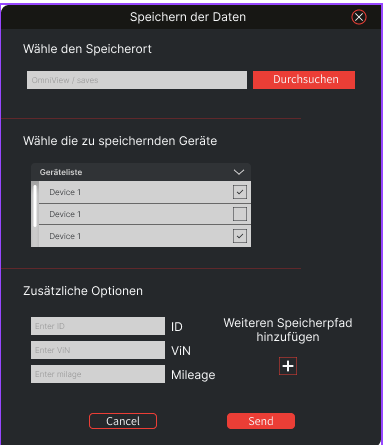
\includegraphics[width=.9\textwidth]{assets/pictures/Popupwindow_png.png}
    \caption[]{A visual representation of a popupwindow}
    \label{fig:popupwindow}
    \end{figure}


\subsubsection{Design of Buttons in Popup Windows}\label{cap:Designprinciples_PopupButtons}

Within Popup Windows in OmnAI View, buttons are designed with careful consideration for user interaction, ensuring a cohesive and intuitive experience:

\begin{itemize}
    \item \textbf{Cancel Buttons:} Cancel buttons exhibit a red border that becomes lighter when hovered. When clicked, the intensity increases for user feedback.
    
    \item \textbf{Save Buttons:} Save buttons are entirely red, with a lighter shade when hovered. Clicking on these buttons increases the intensity, accompanied by a black border for visual emphasis.
    
    \item \textbf{Other Buttons:} Buttons, excluding cancel and save, follow the standard Button or RadioButton design principles, maintaining consistency within the interface.
\end{itemize}

These button designs aim to provide users with a clear visual cue for interaction, ensuring a smooth and predictable experience within the Popup Windows of OmnAI View.

\subsection{Design of Icon Buttons}

Icon Buttons are presented as squares. Each Icon Button is adorned with a unique white symbol on a black background. On hover, they exhibit a red border. Upon clicking, the border disappears, and the white symbol turns red.

The corresponding icons are showcased in Fig. \ref{fig: IconImages}.

\begin{figure}
    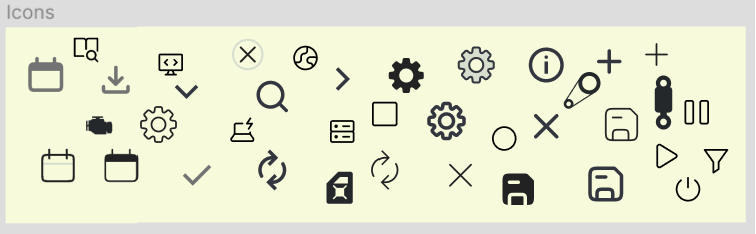
\includegraphics[width=.7\textwidth]{assets/pictures/Icons.png}
    \caption[]{The used Icons in the OmnAI View application}
    \label{fig: IconImages}
\end{figure}

\subsection{Design of a Drop-Down Menu with Checkmarks}

A drop-down menu with checkmarks is visualized in Fig. \ref{fig: DragandDropwithCheckmarks}. The boxes feature a black background with a red border. Hovering over them results in a lighter red border and box. Upon clicking, a red checkmark is displayed within the box.

\begin{figure}
    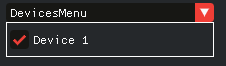
\includegraphics[width=.5\textwidth]{assets/pictures/DropDownMenu.png}
    \caption[]{The used DropDownMenu Design in the OmnAI View application}
    \label{fig: DragandDropwithCheckmarks}
\end{figure}

\subsection{Sidebar Design}

The sidebar backdrop adopts a black hue with the AI logo positioned at the top. The Text color is set to white. 
In the sidebarmenu Buttons and Treenodes exist. Those are complemented by unique icons, as illustrated in Fig. \ref{fig: SideMenuIcons}.
 When a SidebarMenu-Button is active, its text color turns red. When a measurement is taken, the "Search for new devices" Button Text color turns into a greyed-out state.
  After the measurement resets, the "Search for new devices" Button Text color turns white again. The Buttons of Treenode menus include arrows on the side. 
   When the Button is hovered the background of the Button gets lighter.
 When the Buttons are clicked their arrow inverts und their text color and icon color turn red. 

\begin{figure}
    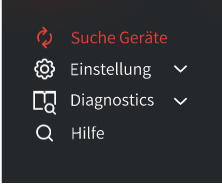
\includegraphics[width=.4\textwidth]{assets/pictures/SideBarMenuButtons.png}
    \caption[]{The used SidBarMenu Buttons in the OmniView application}
    \label{fig: SideMenuIcons}
\end{figure}


    \section{FAQ about the OmniViewSoftware}

    This section provides answers to frequently asked questions about OmniViewSoftware. If you have additional questions, please create an issue where you ask your question, and I will respond to it here.

    \subsection{On which devices should the OmniViewSoftware work?}

    The OmniView Software should work on Linux and Windows systems. The first version only works on computers and laptops and not on mobile devices.

    \subsection{Where can i find the current OmniView Version?}

    The current version of the OmniView Software can be found in the OpenSource skunkforce/OmniView repository.

    \subsection{How will the Software be displayed for the User?}

    The Software is now accessible via a OmniView.exe, in a later process the Software should be opened by an Icon on the Desktop. 

    Certainly! Here is the provided text formatted in LaTeX and translated into English:

    \section{Experiments with one OmniScope}
    The following sections outline potential experiments that can be conducted with one OmniScope in the car mechanic field. 

    \section*{Experiment 1: Battery Voltage Measurement}
    \subsection*{Objective:} Measure the voltage of the vehicle battery to check its state of charge.
    \subsection*{Materials:}
    \begin{enumerate}
        \item Vehicle battery
        \item One OmniScope
        \item Measurement cables
    \end{enumerate}
    \subsection*{Procedure:}
    \begin{enumerate}
        \item Connect the oscilloscope to the battery terminals.
        \item Measure and record the battery voltage.
        \item Analyze the voltage level to assess the state of charge.
    \end{enumerate}

    \section*{Experiment 2: Ignition System Voltage /Second Battery Measurement}
    \subsection*{Objective:} Monitor the ignition voltage to detect ignition pulses and potential misfires.
    \subsection*{Materials:}
    \begin{enumerate}
        \item One OmniScope
        \item Ignition system access (consult vehicle service manual)
        \item Measurement cables
    \end{enumerate}
    \subsection*{Procedure:}
    \begin{enumerate}
        \item Connect the oscilloscope to the ignition system.
        \item Start the engine and observe ignition pulses.
        \item Analyze the waveform for consistency and potential misfires with the corresponding analysis.
    \end{enumerate}

    \section*{Experiment 3: Lambda Probe Voltage Measurement}
    \subsection*{Objective:} Measure the voltage of the Lambda probe to monitor oxygen content in exhaust gas.
    \subsection*{Materials:}
    \begin{enumerate}
        \item Vehicle with Lambda probe
        \item One OmniScope
        \item Measurement cables
    \end{enumerate}
    \subsection*{Procedure:}
    \begin{enumerate}
        \item Connect the oscilloscope to the Lambda probe signal wire.
        \item Start the engine and observe the Lambda probe voltage.
        \item Analyze the voltage fluctuations to assess exhaust gas composition with the corresponding analysis.
    \end{enumerate}

    \section*{Experiment 4: Alternator Voltage Measurement}
    \subsection*{Objective:} Check the voltage output of the alternator to ensure proper charging.
    \subsection*{Materials:}
    \begin{enumerate}
        \item Vehicle with alternator
        \item One OmniScope
        \item Measurement cables
    \end{enumerate}
    \subsection*{Procedure:}
    \begin{enumerate}
        \item Connect the oscilloscope to the alternator output.
        \item Start the engine and observe the alternator voltage.
        \item Analyze the waveform to confirm proper charging operation.
    \end{enumerate}

    \section*{Experiment 5: Starter System Voltage Analysis}
    \subsection*{Objective:} Analyze the voltage during the starting process to detect starter issues.
    \subsection*{Materials:}
    \begin{enumerate}
        \item Vehicle with starter system
        \item One OmniScope
        \item Measurement cables
    \end{enumerate}
    \subsection*{Procedure:}
    \begin{enumerate}
        \item Connect the oscilloscope to the starter system.
        \item Start the engine and observe the voltage during the starting process.
        \item Analyze the waveform for abnormalities indicating starter issues with the corresponding analysis.
    \end{enumerate}

    \section*{Experiment 6: Crankshaft Sensor Voltage Measurement}
    \subsection*{Objective:} Measure the voltage of the crankshaft sensor to obtain precise information about the crankshaft position.
    \subsection*{Materials:}
    \begin{enumerate}
        \item Vehicle with crankshaft sensor
        \item Omniscope
        \item Measurement cables
    \end{enumerate}
    \subsection*{Procedure:}
    \begin{enumerate}
        \item Connect the Omniscope to the crankshaft sensor signal wire.
        \item Start the engine and observe the crankshaft sensor voltage.
        \item Analyze the waveform to determine accurate crankshaft position information.
    \end{enumerate}

    \section*{Experiment 7: Camshaft Sensor Voltage Measurement}
    \subsection*{Objective:} Analyze the voltage of the camshaft sensor to monitor the camshaft position.
    \subsection*{Materials:}
    \begin{enumerate}
        \item Vehicle with camshaft sensor
        \item Omniscope
        \item Measurement cables
    \end{enumerate}
    \subsection*{Procedure:}
    \begin{enumerate}
        \item Connect the Omniscope to the camshaft sensor signal wire.
        \item Start the engine and observe the camshaft sensor voltage.
        \item Analyze the waveform for accurate camshaft position monitoring.
    \end{enumerate}

    \section*{Experiment 8: Coolant Temperature Sensor Voltage Measurement}
    \subsection*{Objective:} Measure the voltage of the coolant temperature sensor to identify potential overheating issues.
    \subsection*{Materials:}
    \begin{enumerate}
        \item Vehicle with coolant temperature sensor
        \item Omniscope
        \item Measurement cables
    \end{enumerate}
    \subsection*{Procedure:}
    \begin{enumerate}
        \item Connect the Omniscope to the coolant temperature sensor signal wire.
        \item Start the engine and observe the coolant temperature sensor voltage.
        \item Analyze the waveform for abnormalities indicating potential overheating.
    \end{enumerate}



    \section{Experiments with two OmniScopes}
    The following sections outline potential experiments that can be conducted with two OmniScopes. 
    These experiments aim to provide a comprehensive understanding of how to effectively utilize OmniScopes for various purposes, offering a broad overview of their functionalities.
    \section*{Experiment 1: Crankshaft and Camshaft Sensor}
    \subsection*{Objective:} Capture voltage waveforms from crankshaft and camshaft sensors, determine phase shifts, and analyze irregularities.
    \subsection*{Materials:}
    \begin{enumerate}
        \item Engine test bench with crankshaft and camshaft sensors
        \item Oscilloscope
        \item Measurement cables
        \item Computer for data analysis
    \end{enumerate}
    \subsection*{Procedure:}
    \begin{enumerate}
        \item Start the engine and bring it to idle speed.
        \item Connect the oscilloscope to the crankshaft and camshaft sensors.
        \item Record the voltage waveforms of both sensors.
        \item Measure the phase shift between the curves or start the "crankshaft and camshaft" analysis.
        \item Analyze irregularities in the curves and document them or look at the analysis results.
    \end{enumerate}

    \section*{Experiment 2: RLC Circuit and Voltage Measurement}
    \subsection*{Objective:} Compare voltages across different components of an RLC circuit.
    \subsection*{Materials:}
    \begin{enumerate}
        \item RLC circuit
        \item AC power source
        \item Oscilloscope
        \item Measurement cables
    \end{enumerate}
    \subsection*{Procedure:}
    \begin{enumerate}
        \item Assemble the RLC circuit according to the circuit diagram.
        \item Connect the AC power source.
        \item Use the oscilloscope to measure voltages across resistance (R), inductor (L), and capacitor (C).
        \item Record and compare the data or use one of the RLC analysis.
    \end{enumerate}

    \section*{Experiment 3: Series Resonant Circuit at Resonance Frequency}
    \subsection*{Objective:} Compare voltages in a series resonant circuit with different resistances and determine the resonance frequency.
    \subsection*{Materials:}
    \begin{enumerate}
        \item Series resonant circuit
        \item AC power source
        \item Resistors of different values
        \item Oscilloscope
        \item Measurement cables
    \end{enumerate}
    \subsection*{Procedure:}
    \begin{enumerate}
        \item Build the series resonant circuit.
        \item Insert various resistors.
        \item Use the oscilloscope to measure voltages and note the data.
        \item Determine the resonance frequency for each resistance.
    \end{enumerate}

    \section*{Experiment 4: Comparison of Two Voltages on a Board}
    \subsection*{Objective:} Compare input and output voltages, verify the correct voltage at a component.
    \subsection*{Materials:}
    \begin{enumerate}
        \item Electronic board with input and output interfaces
        \item Voltage meter
        \item Oscilloscope
        \item Measurement cables
    \end{enumerate}
    \subsection*{Procedure:}
    \begin{enumerate}
        \item Connect the board.
        \item Measure input and output voltages.
        \item Verify the correctness of the voltages.
        \item Optional: Measure the voltage at specific components.
    \end{enumerate}

    \section*{Experiment 5: Temporal Comparison of Coaxial Cable Reflection}
    \subsection*{Objective:} Temporal comparison of reflections in two coaxial cables.
    \subsection*{Materials:}
    \begin{enumerate}
        \item Two coaxial cables
        \item Pulse source
        \item Oscilloscope
        \item Measurement cables
    \end{enumerate}
    \subsection*{Procedure:}
    \begin{enumerate}
        \item Connect the pulse source to the first coaxial cable.
        \item Record the reflection.
        \item Connect the second coaxial cable and compare the reflections or use the coaxial cables analysis.
    \end{enumerate}

    \section*{Experiment 6: Verification of Serial Communication Protocols}
    \subsection*{Objective:} Measure the time intervals between bits.
    \subsection*{Materials:}
    \begin{enumerate}
        \item Device with serial interface
        \item Logic analyzer or oscilloscope
        \item Measurement cables
    \end{enumerate}
    \subsection*{Procedure:}
    \begin{enumerate}
        \item Connect the device to the measuring device.
        \item Initiate the transmission.
        \item Measure the time intervals between the bits.
    \end{enumerate}

    \section*{Experiment 7: Comparison Between Noisy and Clean Signals}
    \subsection*{Objective:} Compare signals on a functioning and a defective device.
    \subsection*{Materials:}
    \begin{enumerate}
        \item Functioning and defective devices
        \item Oscilloscope
        \item Measurement cables
    \end{enumerate}
    \subsection*{Procedure:}
    \begin{enumerate}
        \item Measure the signal on both devices.
        \item Document differences in noisy and clean signals or use the corresponding analysis.
    \end{enumerate}

    \section*{Experiment 8: Analysis of High-pass and Low-pass Filters}
    \subsection*{Objective:} Voltage analysis before and after high-pass and low-pass filters.
    \subsection*{Materials:}
    \begin{enumerate}
        \item High-pass and low-pass filters
        \item AC power source
        \item Oscilloscope
        \item Measurement cables
    \end{enumerate}
    \subsection*{Procedure:}
    \begin{enumerate}
        \item Integrate the filters into the circuit.
        \item Measure the voltage before and after the filters.
        \item Document the effect of the filters.
    \end{enumerate}

    \section*{Experiment 9: Battery Measurement}
    \subsection*{Objective:} Compare battery voltage and generator voltage.
    \subsection*{Materials:}
    \begin{enumerate}
        \item Battery
        \item Generator
        \item Voltmeter
        \item Measurement cables
    \end{enumerate}
    \subsection*{Procedure:}
    \begin{enumerate}
        \item Connect the battery and the generator.
        \item Measure the voltages and compare them.
    \end{enumerate}

    These experiment instructions serve as general guidelines. Please observe safety regulations and specific requirements for the devices and materials used.


%\subsection{Data upload window}

%The upload window should be an extra window that does not overlap with the datawindow. It should contain an upload button and an exit button. The user should be able to put in the 
%current dataset or another dataset from their database. 
%The window should contain fields where the user can put in 
%\begin{itemize}
%    \item the analysis type
%    \item the base data like the workplace of the measurement
%    \item the reasons for the measurement
%    \item if the measurement shows expected course or not 
%\end{itemize}



%\subsection{Help menu}

%The Helpmenu should contain 
%\begin{itemize}
%    \item a link to our ous
%    \item a link to an Tutorial website
%\end{itemize}


\printglossaries

\end{document}